\section{Analysis}\label{sec:dns_analysis} % TODO Better section name?

\todo{fill out...}
We conducted several types of analysis on the \dns data...

\subsection{Distance Normalization}
One of the initial steps in processing the data collected involved adding an additional field for \rtt normalized by the distance between the points being connected. As mentioned earlier in this report, by normalizing for distance, we can form another measurement that allows for analysis of connectivity as related to the \textit{ideal} speed of connection, the speed of light.

Additionally, calculating the speed of the connection, not just the total \rtt, allowed us to filter out measurements that were faster than the speed of light. Such measurements were likely the result of anomalous latency readings, causing the calculated \rtt to be far lower than physically possible. In total, this initial filter eliminated 418,625 measurements (7.5\%) from the total dataset.

\subsection{Raw Data Characteristics}

\subsubsection{True RTT}
\todo{Discuss these}
\begin{figure}[H]
    \centering
    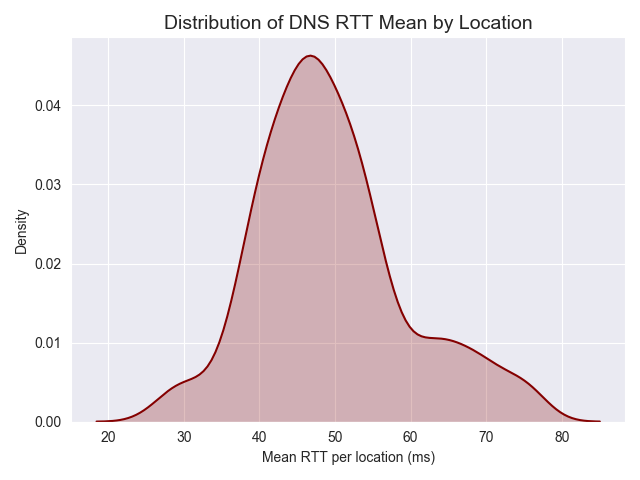
\includegraphics[width=\textwidth]{images/dns/dist_raw_data/dns_rtt_mean_distribution.png}
    \caption{DNS RTT Mean Distribution}
    \label{fig:dns_analytics_mean_dist}
\end{figure}

\begin{figure}[H]
    \centering
    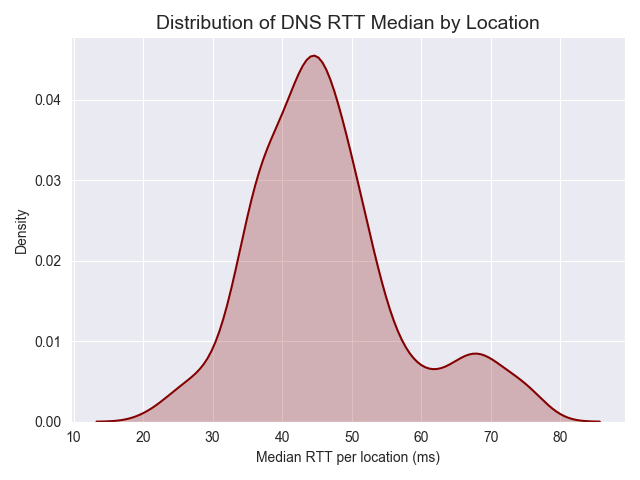
\includegraphics[width=\textwidth]{images/dns/dist_raw_data/dns_rtt_median_distribution.png}
    \caption{DNS RTT Median Distribution}
    \label{fig:dns_analytics_median_dist}
\end{figure}

\begin{figure}[H]
    \centering
    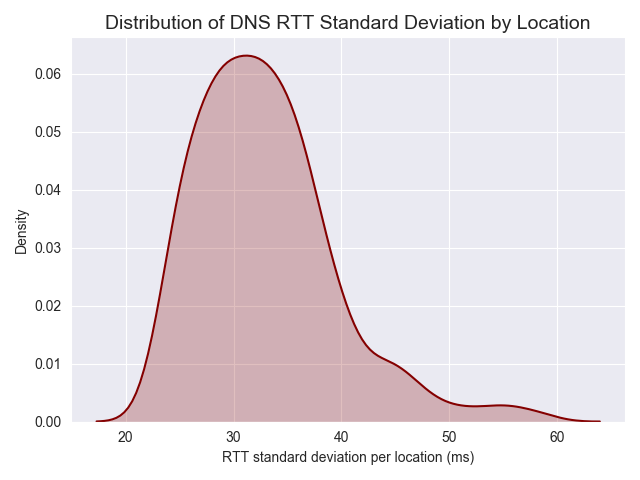
\includegraphics[width=\textwidth]{images/dns/dist_raw_data/dns_rtt_stdev_distribution.png}
    \caption{DNS RTT Standard Deviation Distribution}
    \label{fig:dns_analytics_stdev_dist}
\end{figure}

\begin{figure}[H]
    \centering
    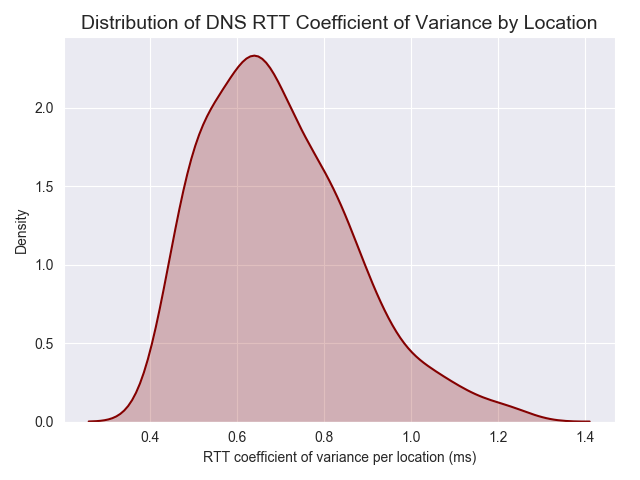
\includegraphics[width=\textwidth]{images/dns/dist_raw_data/dns_rtt_cv_distribution.png}
    \caption{DNS RTT CV Distribution}
    \label{fig:dns_analytics_cv_dist}
\end{figure}

\subsubsection{Normalized RTT}
\todo{Discuss these}
\begin{figure}[H]
    \centering
    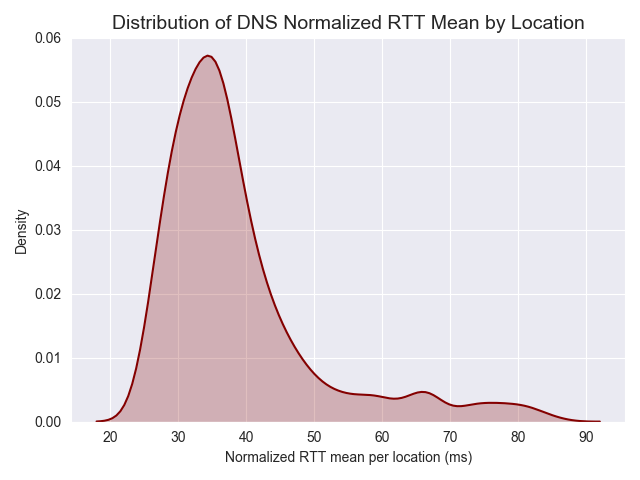
\includegraphics[width=\textwidth]{images/dns/dist_raw_data/dns_norm_rtt_mean_distribution.png}
    \caption{DNS Normalized RTT Mean Distribution}
    \label{fig:dns_analytics_norm_mean_dist}
\end{figure}

\begin{figure}[H]
    \centering
    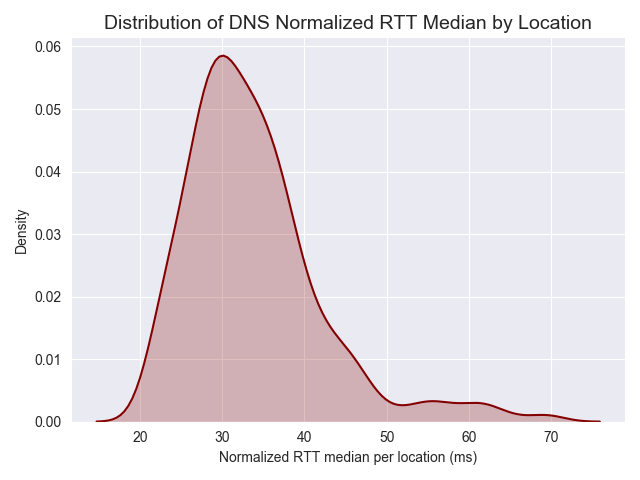
\includegraphics[width=\textwidth]{images/dns/dist_raw_data/dns_norm_rtt_median_distribution.png}
    \caption{DNS Normalized RTT Median Distribution}
    \label{fig:dns_analytics_norm_median_dist}
\end{figure}

\begin{figure}[H]
    \centering
    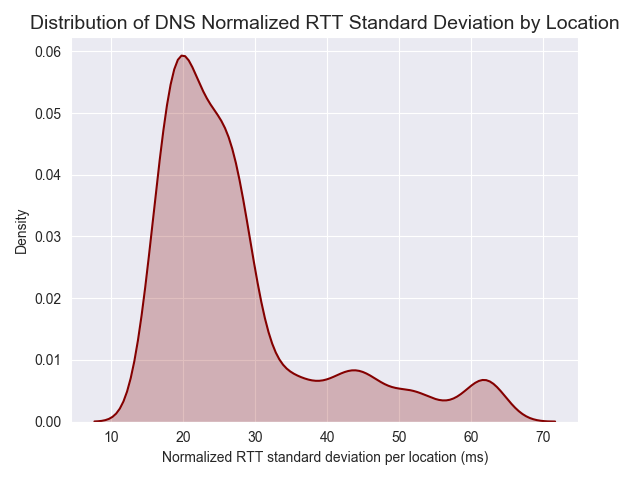
\includegraphics[width=\textwidth]{images/dns/dist_raw_data/dns_norm_rtt_stdev_distribution.png}
    \caption{DNS Normalized RTT Standard Deviation Distribution}
    \label{fig:dns_analytics_norm_stdev_dist}
\end{figure}

\begin{figure}[H]
    \centering
    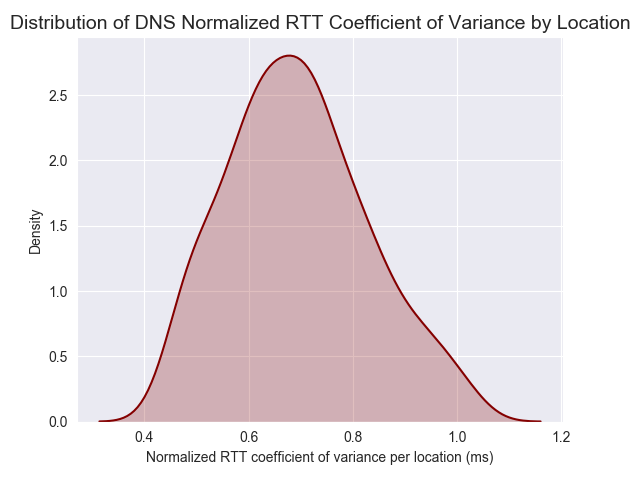
\includegraphics[width=\textwidth]{images/dns/dist_raw_data/dns_norm_rtt_cv_distribution.png}
    \caption{DNS Normalized RTT CV Distribution}
    \label{fig:dns_analytics_norm_cv_dist}
\end{figure}

\subsection{Heat Map(s)}

\todo{Add True RTT heatmap}
Discuss heatmap here...


\begin{figure}[H]
    \centering
    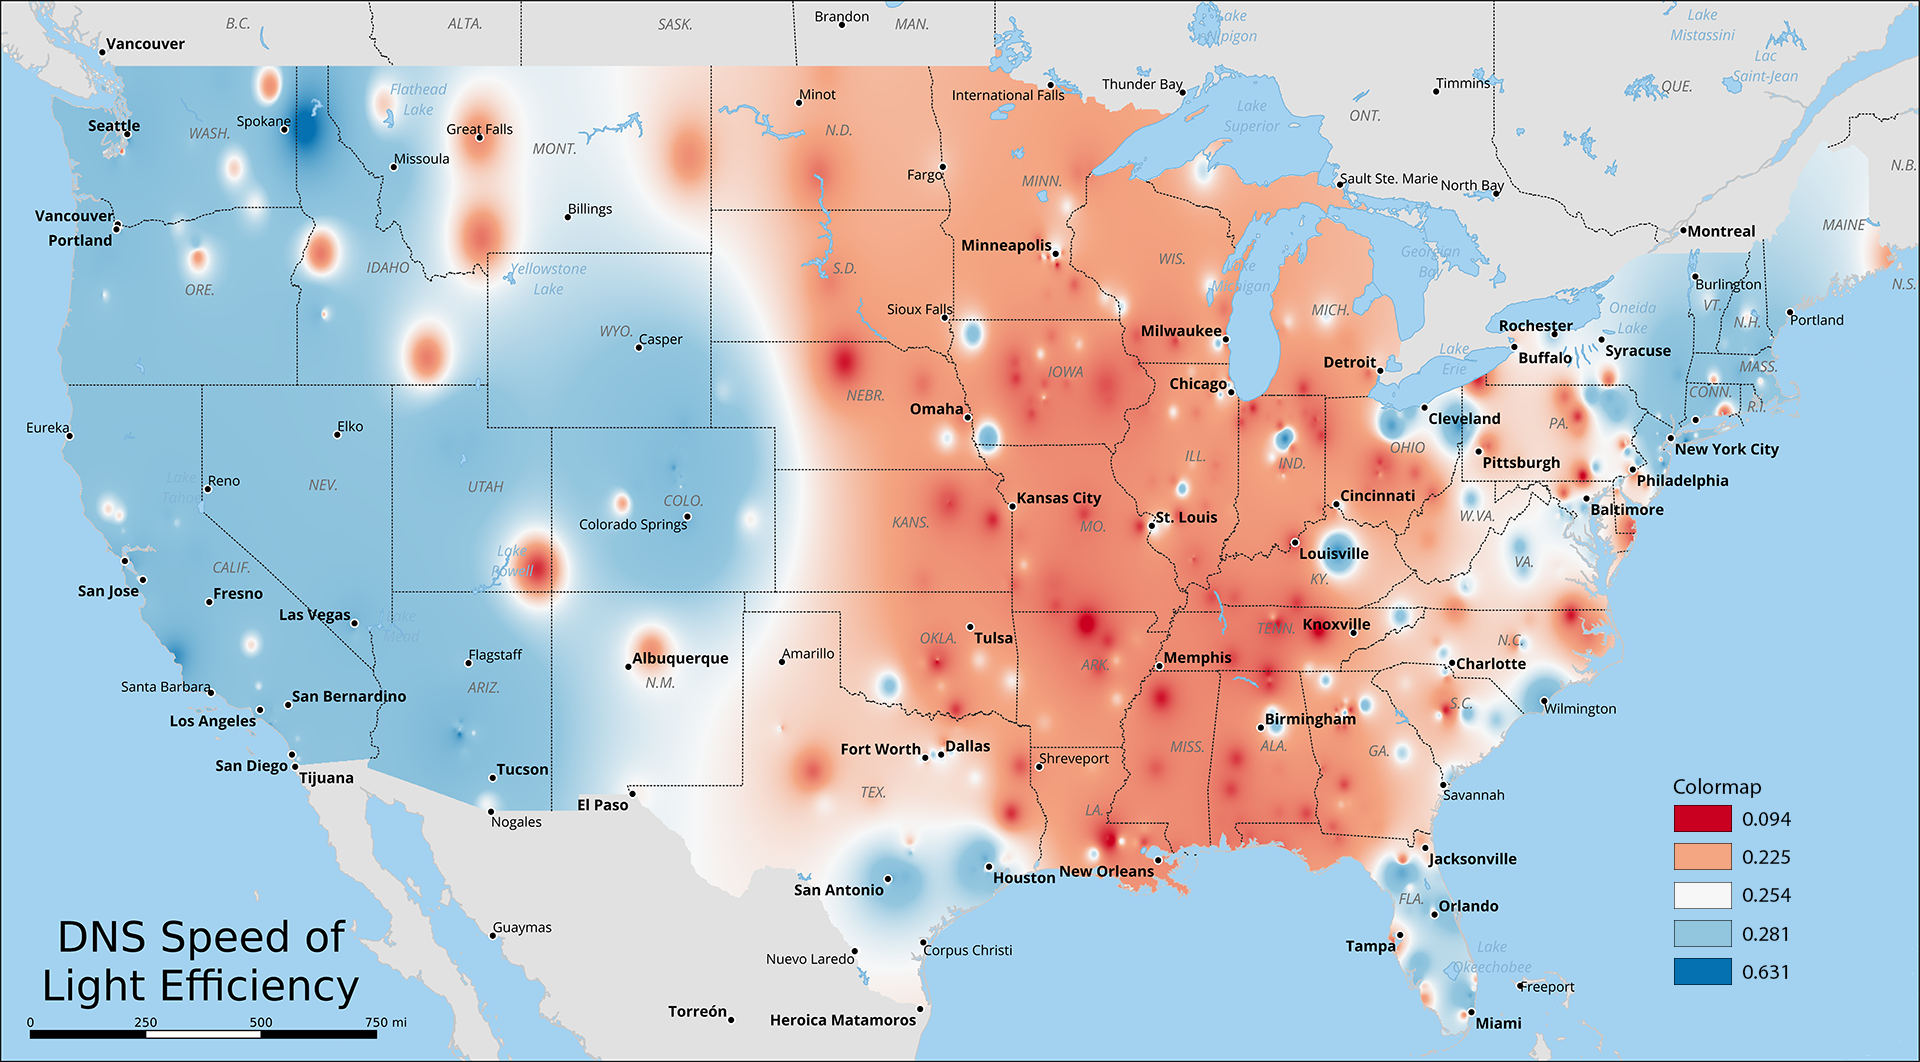
\includegraphics[width=\textwidth]{images/dns/heatmaps/dns_speed_of_light_idw.png}
    \caption{DNS Normalized RTT Heatmap}
    \label{fig:dns_normalized_rtt_heatmap}
\end{figure}

\subsection{Aggregation by Server Pairs}
Since there we multiple data points for each recursive-authoritative server pair, the first step in aggregating the data was to aggregate by these server pairs. To do this, we removed points within each pair that had a z-score greater than a given threshold \texttt{z} as these were considered outliers within their pairs. We then computed the \cv of each pair with the remaining values and discarded any pairs with a result greater than a given threshold \texttt{v} - these pairs did not have consistent measurements and were considered unreliable.

\begin{table}[h]
    \centering
    \begin{tabular}{ |l|l|l|  }
     \hline
     \multicolumn{3}{|c|}{DNS Z-score filtering} \\
     \hline
      & True \rtt records dropped & Normalized \rtt records dropped \\
     \hline
      \texttt{z=3} & 92,553/5,188,421 (1.8\%) & 63,008/5,188,421 (1.2\%) \\
      \texttt{z=2} & 269,651/5,188,421 (5.2\%) & 237,353‬/5,188,421 (4.6\%) \\
      \texttt{z=1} & 1,362,184/5,188,421 (26.3\%) & 1,389,031‬/5,188,421 (26.8\%) \\
     \hline
    \end{tabular}
    \caption{DNS Z-score filtering}
    \label{tab:dns_z_filtering}
\end{table}

\todo{Expand}
We chose to proceed with \texttt{z=2}.

\begin{table}[H]
    \centering
    \begin{tabular}{ |p{1.6cm}|p{4cm}|p{4cm}|p{4cm}| }
        \hline
        \multicolumn{4}{|c|}{CV Filtering - Pairs Dropped} \\
        \hline
         & \texttt{z=3} (\texttt{n=381,333}) & \texttt{z=2} (\texttt{n=381,333}) & \texttt{z=1} (\texttt{n=381,333}) \\
        \hline
        \texttt{v=0.05} & 193,099 (50.6\%)  & 167,618 (44.0\%) & ‭92,799 (24.3\%) \\
        \texttt{v=0.10} & 111,294 (29.2\%) & 92,023 (24.1\%) & 40,889 (10.7\%)‬\\
        \texttt{v=0.20} & 52,239 (13.7\%) &  40,353 (10.6\%) & 13,262 (3.5\%)\\
        \texttt{v=0.50} & 9,330 (2.4\%) &  6,333 (1.7\%) & 1,809 (0.5\%)\\
        \texttt{v=1.00} & 1,741 (0.5\%) &    766 (0.2\%) & 176 (~0.0\%) \\
        \hline
    \end{tabular}
    \caption{True RTT DNS Pair CV Filtering}
    \label{tab:dns_unnorm_cv_filtering}
\end{table}

\begin{table}[H]
    \centering
    \begin{tabular}{ |p{1.6cm}|p{4cm}|p{4cm}|p{4cm}| }
        \hline
        \multicolumn{4}{|c|}{CV Filtering - Pairs Dropped} \\
        \hline
         & \texttt{z=3} (\texttt{n=382,963}) & \texttt{z=2} (\texttt{n=382,963}) & \texttt{z=1} (\texttt{n=382,963}) \\
        \hline
        \texttt{v=0.05} & 192,522 (50.3\%) & 166,514 (43.5\%) & 87,383 (22.8\%) \\
        \texttt{v=0.10} & 109,493 (28.6\%) & 89,906 (23.5\%) & 35,553 (9.3\%) \\
        \texttt{v=0.20} & 48,414 (12.6\%) & 37,623 (9.8\%) & 10,579 (2.8\%) \\
        \texttt{v=0.50} & 6,304 (1.6\%) & 4,570 (1.2\%) & 1,314 (0.3\%) \\
        \texttt{v=1.00} & 1,038 (0.3\%) &    415 (0.1\%) & 126 (~0.0\%) \\  
        \hline
    \end{tabular}
    \caption{Normalized RTT DNS Pair CV Filtering}
    \label{tab:dns_norm_cv_filtering}
\end{table}

We chose to proceed with \texttt{v=1.0}, which left the vast majority of pairs in the dataset excluding only the most inconsistent measurements. The reasoning behind this is that we aren't just interested in stable connections - so we left potentially unstable or inconsistent measurements in the dataset.

\subsubsection{Data Characteristics}

\subsection{Aggregating Pairs by Recursive State}

One option to further aggregate the pair data is to group it by the location of the recursive server in each pair. This results in a list of \rtts, either true or normalized by distance, that can be aggregated into a single value for each state. This is one way of making comparisons between states.

\subsubsection{Initial State Rankings}

\Cref{tab:dns_only_recursive_initial_state_rankings} shows the results of ranking states by the median of each measurement in that state. There are two different rankings, one each for the true \rtt and the distance normalized \rtt, based on data filtered with \texttt{z=2} and \texttt{v=1.0}. As with all \dns data, there is no ranking for Rhode Island.

\begin{longtable}{lrr||lrr}
% \toprule
  \multicolumn{3}{c||}{\textbf{True RTT}} & \multicolumn{3}{c}{\textbf{Normalized RTT}} \\
     \textbf{State} &  \textbf{Rank} & \textbf{(ms)} & \textbf{State} & \textbf{Rank} & \textbf{(km/ms)} \\
\midrule
\endhead
\midrule
\multicolumn{6}{r}{{Continued on next page}} \\
\midrule
\endfoot
% \bottomrule
\endlastfoot
        WY &    1 &  30.0 &             HI &    1 &  91.0 \\
        VA &    2 &  31.0 &             WY &    2 &  54.5 \\
        DC &    2 &  31.0 &             AK &    3 &  47.4 \\
        WV &    4 &  32.0 &             CA &    4 &  45.5 \\
        NY &    4 &  32.0 &             OR &    5 &  43.9 \\
        NJ &    6 &  33.0 &             NV &    6 &  43.7 \\
        MD &    7 &  34.0 &             CO &    7 &  43.6 \\
        SC &    8 &  34.5 &             NY &    8 &  43.0 \\
        CO &    9 &  38.0 &             UT &    9 &  42.7 \\
        NH &   10 &  38.5 &             ID &   10 &  42.0 \\
        IL &   11 &  39.0 &             WA &   11 &  41.8 \\
        MI &   12 &  40.0 &             NH &   12 &  41.7 \\
        PA &   12 &  40.0 &             AZ &   13 &  41.0 \\
        WI &   12 &  40.0 &             NJ &   14 &  40.9 \\
        NC &   15 &  41.0 &             MA &   15 &  40.7 \\
        TX &   16 &  42.0 &             VA &   16 &  37.1 \\
        MA &   16 &  42.0 &             FL &   17 &  37.0 \\
        OH &   16 &  42.0 &             TX &   18 &  36.8 \\
        IN &   19 &  43.0 &             MD &   19 &  36.4 \\
        GA &   19 &  43.0 &             DC &   20 &  35.8 \\
        MN &   21 &  45.0 &             SC &   21 &  34.6 \\
        OK &   22 &  46.0 &             CT &   22 &  33.6 \\
        MO &   22 &  46.0 &             PA &   23 &  33.3 \\
        LA &   22 &  46.0 &             NC &   24 &  32.4 \\
        AR &   22 &  46.0 &             MT &   25 &  32.0 \\
        CT &   22 &  46.0 &             VT &   26 &  31.6 \\
        FL &   27 &  47.0 &             MI &   27 &  31.5 \\
        IA &   28 &  48.0 &             WI &   28 &  30.6 \\
        KY &   29 &  49.0 &             WV &   29 &  30.6 \\
        NE &   30 &  49.5 &             NM &   30 &  30.4 \\
        UT &   31 &  50.0 &             MN &   31 &  30.0 \\
        VT &   32 &  51.0 &             ME &   32 &  29.8 \\
        TN &   33 &  52.0 &             GA &   33 &  29.6 \\
        AL &   34 &  53.0 &             ND &   34 &  29.4 \\
        AZ &   34 &  53.0 &             LA &   35 &  29.3 \\
        DE &   34 &  53.0 &             OK &   36 &  28.9 \\
        NV &   34 &  53.0 &             SD &   37 &  28.6 \\
        ID &   38 &  54.0 &             NE &   38 &  28.3 \\
        SD &   39 &  56.0 &             IL &   39 &  28.1 \\
        KS &   39 &  56.0 &             DE &   40 &  27.6 \\
        ND &   41 &  59.0 &             MO &   41 &  26.4 \\
        CA &   42 &  59.5 &             AR &   42 &  26.2 \\
        NM &   43 &  60.0 &             OH &   43 &  25.4 \\
        HI &   43 &  60.0 &             IA &   44 &  25.0 \\
        MS &   45 &  62.0 &             AL &   45 &  24.5 \\
        OR &   46 &  65.0 &             IN &   46 &  24.4 \\
        WA &   47 &  67.0 &             KS &   47 &  22.9 \\
        ME &   48 &  67.5 &             KY &   48 &  21.9 \\
        MT &   49 &  71.0 &             TN &   49 &  21.6 \\
        AK &   50 &  99.2 &             MS &   50 &  20.4 \\
        RI &   -- &    -- &             RI &   -- &    -- \\
        \caption{Initial State Rankings -- Recursive Location Aggregation}
        \label{tab:dns_only_recursive_initial_state_rankings}
\end{longtable}


Notably, \cref{tab:dns_only_recursive_initial_state_rankings} indicates that Wyoming ranks in the top five for both rankings. ...

Also, the rankings show that while Hawaii and Alaska rank near or at the bottom for true \rtt, both states appear near the top of the normalized ranking. This shows that while the some states, Alaska and Hawaii in particular, may be inherently unconnected from the rest of the United States, the quality of their connection could be relatively high and merely dominated by sheer distances.

\subsubsection{Evaluating State Rankings}

To determine the validity of the rankings proposed above we used the Kruskal-Wallis test to determine whether there was evidence that datasets for different states came from different distributions. If we cannot reject the null hypothesis that they are from the same distribution, we cannot rank them in distinct positions. After running Kurskals between the datasets for each of the 49 states + DC, we used a p value threshold of 0.05 to determine if we could differentiate two states from each other. 

True \rtt:
\begin{figure}[H]
    \centering
    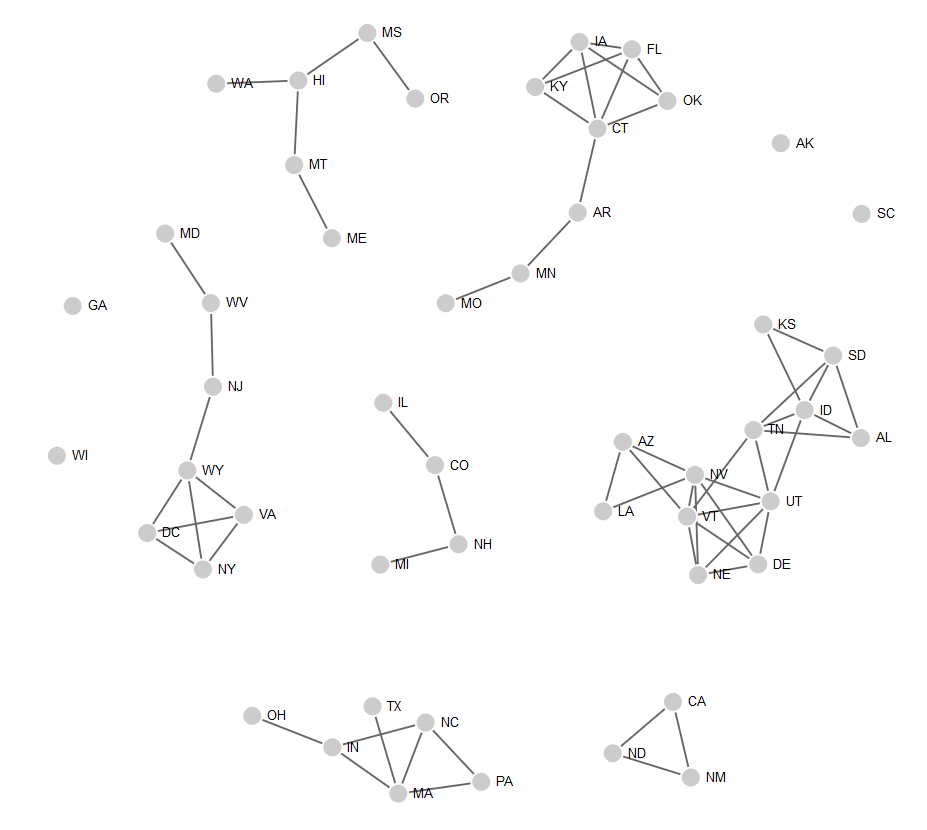
\includegraphics[width=\textwidth]{images/dns/kruskals_analysis_no_auth_agg/rtt/graph.png}
    \caption{DNS True RTT Indistinguishable States Graph}
    \label{fig:dns_true_rtt_indistinguishable_states_graph}
\end{figure}

\textit{Notes for writeup: "big dipper" is the top 7 states. Backwards L is 9-12 (SC is \#8). Group with MO as tail spans 21-29 with LA in the middle (distinct) at 22-t. Large cluster spans 30-39. ... AK last}

\begin{figure}[H]
    \centering
    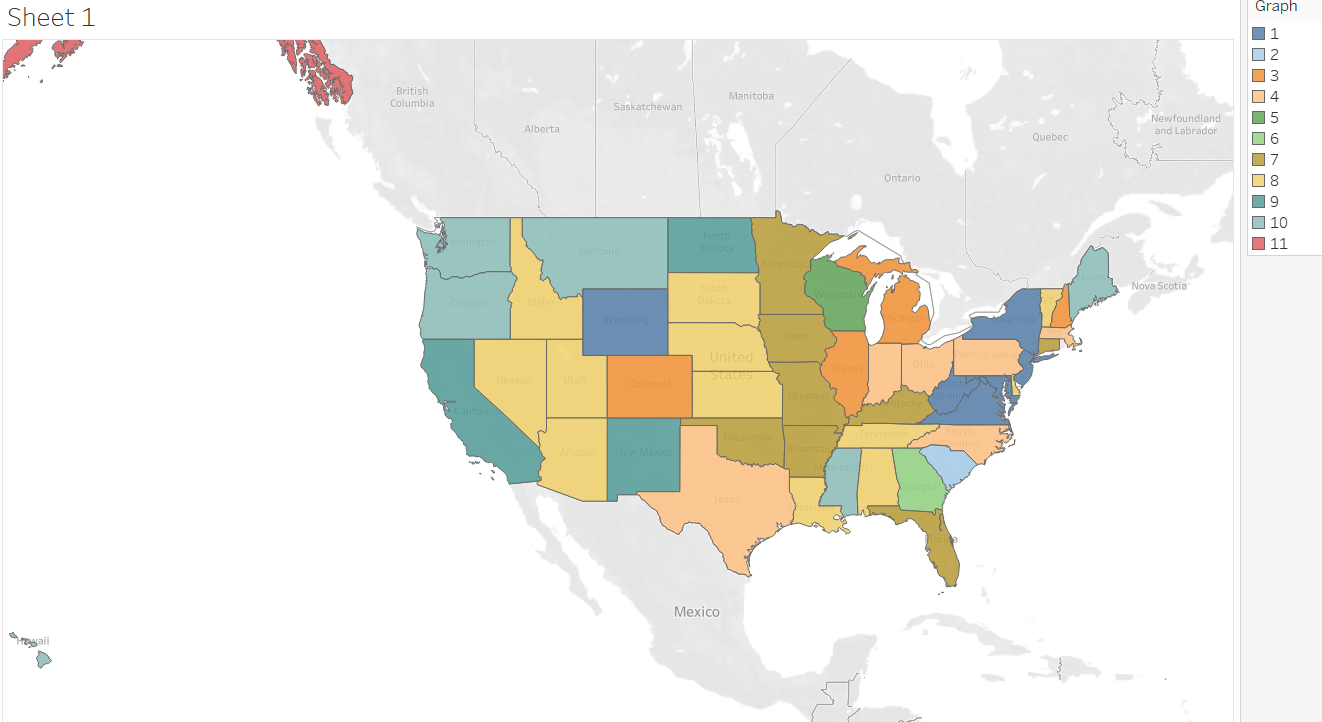
\includegraphics[width=\textwidth]{images/dns/kruskals_analysis_no_auth_agg/rtt/distinct_map1.png}
    \caption{DNS True RTT Indistinguishable States Map}
    \label{fig:dns_true_rtt_indistinguishable_states_map}
\end{figure}

\begin{figure}[H]
    \centering
    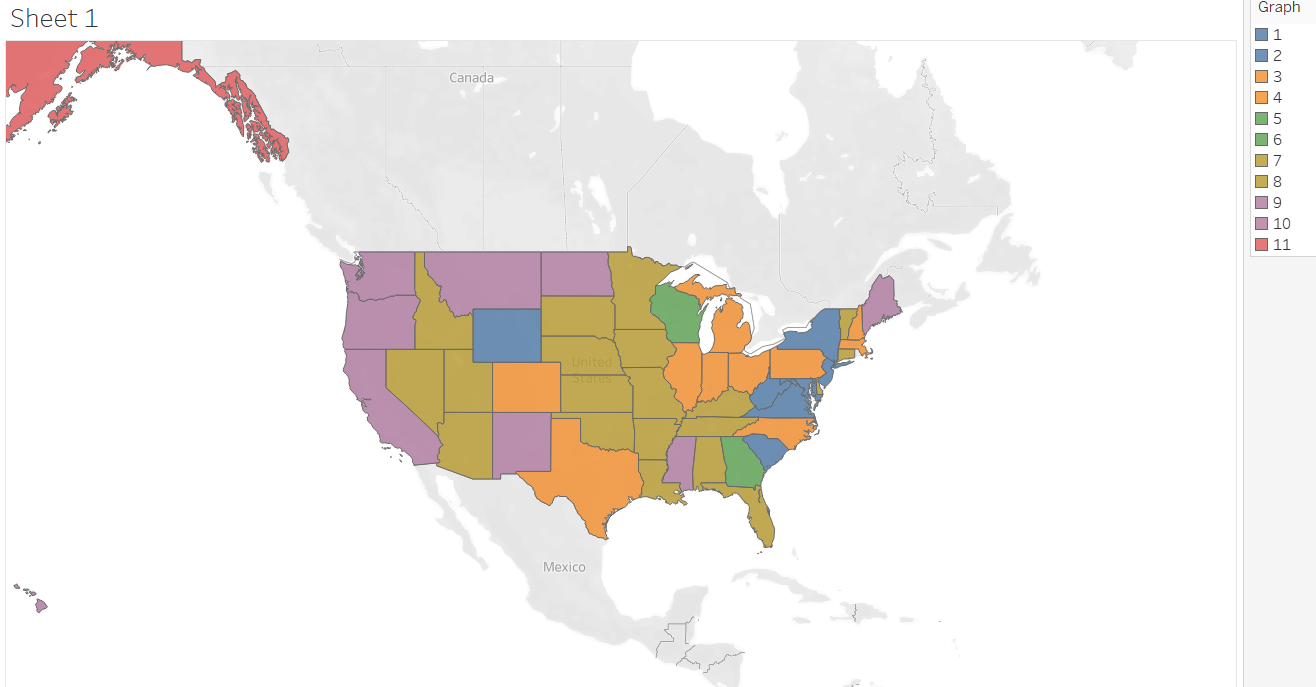
\includegraphics[width=\textwidth]{images/dns/kruskals_analysis_no_auth_agg/rtt/distinct_map2.png}
    \caption{DNS True RTT Indistinguishable States Map Condensed Colors}
    \label{fig:dns_true_rtt_indistinguishable_states_map_condensed_colors}
\end{figure}

\textit{Notes for writeup: second map is colors condensed based on similar groups. Note the big midwest group of 7/8, 4 state cluster 8. Northeast/midatlantic clusters of 1 (outlier for 1: Wyoming). Also: great lakes cluster of 3/4. South is hodgepodge. Pacific is 9/10}

Normalized \rtt:
\begin{figure}[H]
    \centering
    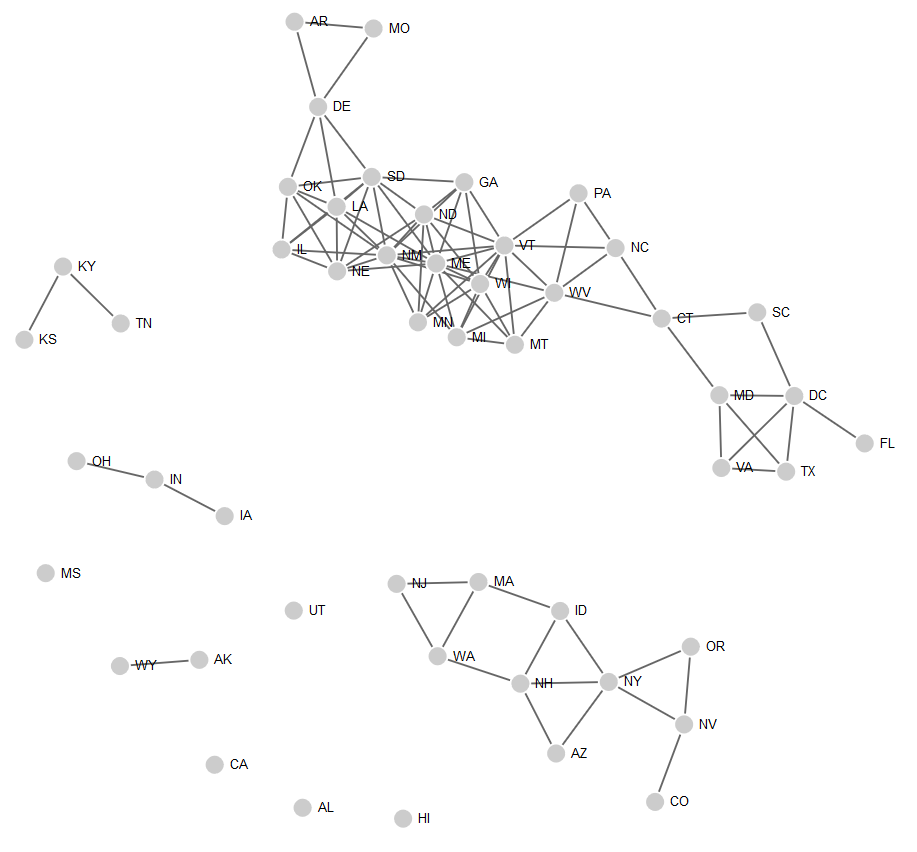
\includegraphics[width=\textwidth]{images/dns/kruskals_analysis_no_auth_agg/rtt_normalized/graph.png}
    \caption{DNS Normalized RTT Indistinguishable States Graph}
    \label{fig:dns_normalized_rtt_indistinguishable_states_graph}
\end{figure}

\textit{Notes for writeup: overall, far messier. More individuals are distinct, but with one much larger group, which dominates the middle of the rankings (16-42 uninterrupted). Hawaii alone at top. Alaska and Wyoming right below. CA independent at 4. Second largest group spans 5-15 with UT in middle at 9 (independent). MS alone at the bottom.}

\begin{figure}[H]
    \centering
    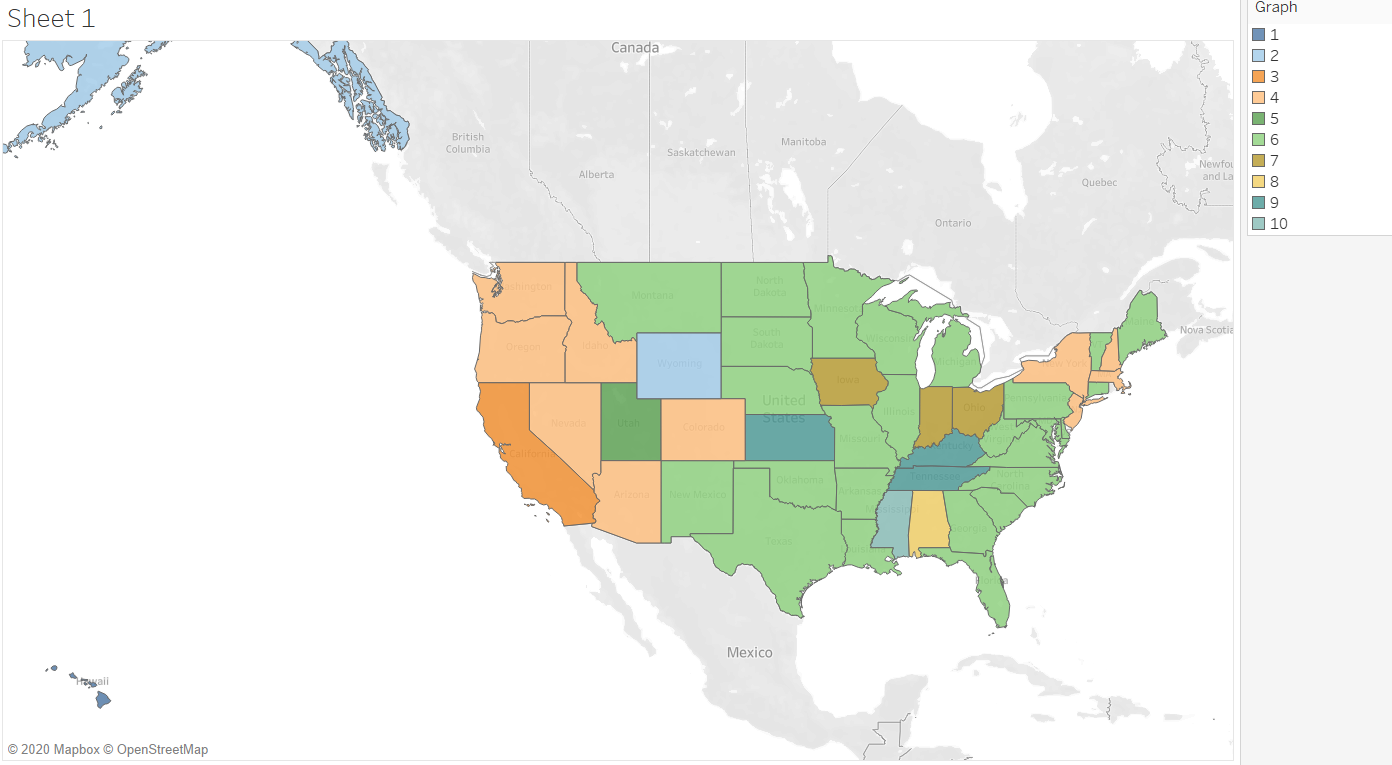
\includegraphics[width=\textwidth]{images/dns/kruskals_analysis_no_auth_agg/rtt_normalized/distinct_map1.png}
    \caption{DNS Normalized RTT Indistinguishable States Map}
    \label{fig:dns_normalized_rtt_indistinguishable_states_map}
\end{figure}

\begin{figure}[H]
    \centering
    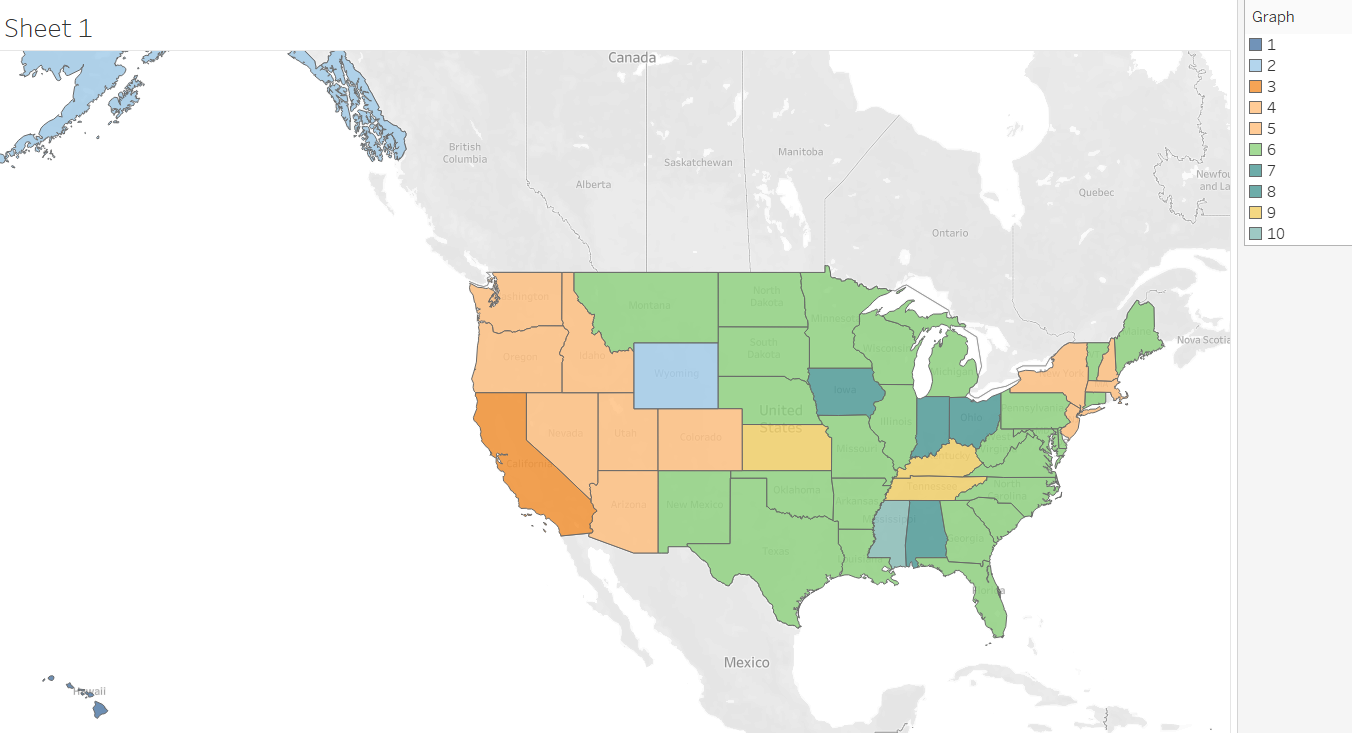
\includegraphics[width=\textwidth]{images/dns/kruskals_analysis_no_auth_agg/rtt_normalized/distinct_map2.png}
    \caption{DNS Normalized RTT Indistinguishable States Map Condensed Colors}
    \label{fig:dns_normalized_rtt_indistinguishable_states_map_consdensed_colors}
\end{figure}

\textit{Notes for writeup: note the western block (4/5) + CA (3) (+WY, AK, HI 1/2). Note the partial Northeast block, also 4/5. Rest is \textit{far less clear}.}



\subsubsection{Aggregation Summary}







\subsection{Aggregation by Authoritative State then Recursive State}

One shortcoming of aggregating pairs directly by the location of the recursive server is that this inherently weights the data by the number of authoritative servers in a single state. To compensate, this analysis method first groups and aggregates by recursive server \textit{and} authoritative server location. Assuming the presence of data for every state, this creates a list of 51 measurements for each state (one for measurements between servers both located in that state, and 50 for each of the other states). These can then be further aggregated into a single value for each state in which each other state is given equal value. We can also add weights to the values based on the authoritative state - for example, by adding a weight based on state population, we create a measurement that values faster connection times to states with greater populations.

\subsubsection{Applying Weights}

\subsubsection{Initial State Rankings}

\todo{Units}
\begin{longtable}{lrr|lrr||lrr|lrr}
\toprule
  \multicolumn{6}{c||}{True RTT} & \multicolumn{6}{c}{Normalized RTT} \\
\multicolumn{3}{c|}{Unweighted} & \multicolumn{3}{c||}{Pop. Weighted} & \multicolumn{3}{c|}{Unweighted} & \multicolumn{3}{c}{Pop. Weighted} \\
     State & Rank & Value &         State & Rank &  Value &          State & Rank &  Value &         State & Rank &  Value \\
\midrule
\endhead
\midrule
\multicolumn{12}{r}{{Continued on next page}} \\
\midrule
\endfoot
\bottomrule
\endlastfoot
        VA &    1 &  39.6 &            WI &    1 &   49.4 &             HI &    1 &  106.9 &            WY &    1 &  147.6 \\
        NY &    2 &  40.3 &            CO &    2 &   49.9 &             WY &    2 &   71.7 &            HI &    2 &  125.4 \\
        WY &    3 &  40.9 &            IL &    3 &   50.0 &             VT &    3 &   50.8 &            VT &    3 &   72.1 \\
        WV &    3 &  40.9 &            WV &    4 &   50.3 &             AK &    4 &   46.8 &            AZ &    4 &   69.1 \\
        MD &    5 &  41.2 &            UT &    5 &   51.0 &             CA &    5 &   46.7 &            CA &    5 &   63.3 \\
        DC &    6 &  42.0 &            MI &    6 &   51.4 &             NV &    6 &   46.2 &            NV &    6 &   60.7 \\
        NJ &    7 &  42.3 &            TX &    7 &   51.5 &             UT &    7 &   46.1 &            CT &    7 &   59.6 \\
        WI &    8 &  43.5 &            MN &    8 &   51.9 &             AZ &    8 &   43.5 &            OR &    8 &   57.6 \\
        IL &    9 &  43.7 &            SC &    9 &   53.8 &             CT &    9 &   43.4 &            UT &    9 &   56.9 \\
        SC &    9 &  43.7 &            NY &   10 &   54.1 &             OR &   10 &   43.3 &            WA &   10 &   52.5 \\
        MI &   11 &  43.8 &            OH &   11 &   54.3 &             WA &   11 &   41.9 &            NM &   11 &   50.1 \\
        CT &   11 &  43.8 &            IN &   12 &   54.4 &             NY &   12 &   40.3 &            AK &   12 &   49.5 \\
        CO &   13 &  44.7 &            VA &   13 &   54.7 &             CO &   13 &   39.8 &            NY &   13 &   49.0 \\
        UT &   14 &  46.4 &            MO &   14 &   54.9 &             NM &   14 &   38.8 &            CO &   14 &   47.0 \\
        NH &   15 &  47.2 &            NJ &   15 &   55.3 &             NH &   15 &   38.7 &            NH &   15 &   46.9 \\
        TX &   15 &  47.2 &            AR &   16 &   56.0 &             VA &   16 &   37.4 &            VA &   16 &   45.8 \\
        PA &   17 &  47.6 &            CT &   17 &   56.1 &             NJ &   17 &   37.3 &            MT &   17 &   45.7 \\
        NC &   18 &  47.7 &            NM &   18 &   56.4 &             TX &   17 &   37.3 &            DC &   18 &   45.6 \\
        MN &   19 &  48.0 &            WY &   19 &   56.9 &             MD &   19 &   37.1 &            NJ &   18 &   45.6 \\
        OH &   20 &  48.8 &            MD &   20 &   57.1 &             FL &   20 &   36.6 &            MD &   20 &   45.1 \\
        AR &   21 &  49.0 &            PA &   20 &   57.1 &             DC &   20 &   36.6 &            SC &   21 &   42.2 \\
        IN &   22 &  49.1 &            LA &   22 &   57.2 &             SC &   22 &   35.8 &            WV &   22 &   41.7 \\
        GA &   23 &  50.1 &            OK &   23 &   57.5 &             MA &   23 &   33.8 &            NE &   23 &   41.2 \\
        LA &   24 &  50.3 &            GA &   23 &   57.5 &             WV &   24 &   33.4 &            MA &   24 &   40.7 \\
        NM &   25 &  50.7 &            IA &   25 &   57.7 &             MT &   25 &   32.8 &            TX &   25 &   40.2 \\
        MO &   26 &  50.9 &            NV &   26 &   57.8 &             LA &   25 &   32.8 &            FL &   26 &   39.7 \\
        MA &   27 &  51.5 &            DC &   27 &   58.4 &             NE &   27 &   32.5 &            MN &   27 &   38.6 \\
        NE &   28 &  51.8 &            NC &   28 &   58.5 &             NC &   28 &   31.7 &            ID &   28 &   38.5 \\
        NV &   29 &  53.0 &            AZ &   29 &   58.7 &             MI &   29 &   31.3 &            PA &   29 &   37.6 \\
        IA &   30 &  53.2 &            NE &   30 &   60.5 &             ID &   30 &   31.1 &            LA &   30 &   37.2 \\
        OK &   30 &  53.2 &            NH &   31 &   61.1 &             GA &   31 &   31.0 &            NC &   31 &   37.1 \\
        FL &   32 &  54.6 &            KY &   32 &   61.3 &             MN &   32 &   30.9 &            GA &   32 &   36.1 \\
        AZ &   33 &  55.2 &            FL &   33 &   62.8 &             WI &   33 &   30.5 &            MI &   33 &   34.5 \\
        KY &   34 &  55.8 &            MA &   33 &   62.8 &             PA &   34 &   30.4 &            WI &   34 &   34.2 \\
        SD &   35 &  58.6 &            SD &   35 &   63.7 &             AR &   35 &   29.2 &            OH &   35 &   34.0 \\
        TN &   36 &  59.1 &            CA &   36 &   64.1 &             IL &   35 &   29.2 &            AR &   36 &   33.9 \\
        AL &   37 &  59.7 &            ND &   37 &   64.3 &             ND &   37 &   28.4 &            IL &   37 &   33.8 \\
        CA &   38 &  60.0 &            AL &   38 &   65.3 &             OK &   38 &   28.1 &            DE &   38 &   33.1 \\
        ND &   39 &  60.9 &            KS &   39 &   65.9 &             ME &   39 &   27.6 &            OK &   39 &   32.3 \\
        KS &   40 &  62.9 &            TN &   39 &   65.9 &             SD &   40 &   27.2 &            ND &   40 &   32.1 \\
        DE &   41 &  63.5 &            DE &   41 &   68.7 &             MO &   41 &   26.4 &            ME &   41 &   31.9 \\
        OR &   42 &  65.1 &            MT &   42 &   71.5 &             AL &   41 &   26.4 &            SD &   42 &   31.1 \\
        WA &   43 &  66.4 &            WA &   43 &   72.3 &             OH &   43 &   26.3 &            MO &   43 &   30.7 \\
        MT &   44 &  67.4 &            MS &   44 &   72.9 &             IN &   44 &   25.4 &            IN &   43 &   30.7 \\
        MS &   45 &  68.8 &            OR &   45 &   74.3 &             IA &   45 &   24.7 &            AL &   45 &   30.5 \\
        HI &   46 &  70.5 &            HI &   46 &   81.6 &             DE &   46 &   24.6 &            IA &   46 &   28.6 \\
        ID &   47 &  74.9 &            ID &   47 &   82.6 &             KY &   47 &   23.0 &            TN &   47 &   28.1 \\
        ME &   48 &  77.8 &            ME &   48 &   85.1 &             TN &   48 &   22.6 &            KY &   48 &   28.0 \\
        VT &   49 &  83.9 &            AK &   49 &  102.9 &             MS &   49 &   22.2 &            MS &   49 &   26.5 \\
        AK &   50 &  99.1 &            VT &   50 &  104.1 &             KS &   50 &   22.1 &            KS &   50 &   25.8 \\
        RI &   -- &    -- &            RI &   -- &     -- &             RI &   -- &     -- &            RI &   -- &     -- \\
        
%         \caption{Initial State Rankings -- Authoritative Location Aggregation}
%         \label{tab:dns_auth_initial_state_rankings}
\end{longtable}

\subsubsection{Evaluating State Rankings}

\subsubsection{Aggregation Summary}












\subsection{DNS Conclusions}